\section{Методы генерации состязательных примеров}
\label{sec:AdversarialGen} \index{AdversarialGen}

\noindent\hspace{0.6cm}Основная идея генерации состязательных примеров для текстов состоит в искажениях символов, слов или целых предложений так, чтобы при этом допускалось либо визуальное сходство, либо семантическое сходство между состязательным примеров и исходным текстом.

\subsection{Символьное искажение}
\label{sec:AdvSymbol}

\noindent\hspace{0.6cm}Подход на уровне символов основан на идее добавления естественных опечаток в слово текста, то есть \textbf{удаление}/\textbf{del}, \textbf{замена}/\textbf{sub}, \textbf{вставка}/\textbf{ins}, согласно его \textbf{WordPiece токенизации} \cite{adversarialgenerating1}, \cite{adversarialgenerating3}. Таким образом, данный метод оперирует \textbf{визуальным сходством} между состязательным примером и исходным текстом. Подход пытается сделать опечатки так, чтобы лексемы искаженного слова, полученные после токенизации, имели минимальное пересечение с лексемами исходного слова. Для подсчета данного пересечения используются метрики расстояния между лексемами слов, в случае если было сгенерировано несколько слов-кандидатов на замену исходному:

\begin{enumerate}
    \item \textbf{Min Token Intersection (MTI)} - Кандидаты с минимальным пересечениям по лексемам остаются. Например, для слова “melodrama” → [’mel’, ’\#\#od’, ’\#\#rama’] мы оставил “melodarma” → [’mel’, ’\#\#oda’, ’\#\#rma’], вместо “melodramas” → [’mel’, ’\#\#od’, ’\#\#rama’, ’\#\#s’];
    \item \textbf{Max Token Count Distance (MTCD)} - Вычисляется разность между количеством лексем до и после Word Piece токенизации. Например, в этом случае для слово «melodrama» → ['mel', '\#\#od', '\#\#rama'] оставляется «nelodrama» →['ne', '\#\#lo', '\#\#dra', '\#\#ma'], вместо "melodarma" → ['mel', '\#\#oda', '\#\#rma'];
    \item \textbf{Min Token Intersection} + \textbf{Max Token Count Distance} (\textbf{MTI} + \textbf{MTCD}) - Если по какой-то из двух выше метрик нельзя выбрать лучшего кандидата, то просматривается ещё другая метрик и уже по ней происходит отбор.
\end{enumerate}

\subsection{Искажение слов}
\label{sec:AdvWord}

\noindent\hspace{0.6cm}Основная идея генерация состязательных примеров на уровне слов заключается в подмене наиболее важного слова некоторым синонимом, чтобы изменения были как можно более естественными, то есть сохранялись исходные морфологические особенности (например, падеж, род и т.д.), тогда в данном случае имеет место \textbf{семантическое сходство}. Таким образом, для достижения данной цели можно применить следующий подход \cite{adversarialgenerating3}:

\begin{enumerate}
    \item Первым делом необходимо выделить наиболее важное слово в тексте и лемматизировать его;
    \item Затем для данного лемматизированного слова надо извлечь его синоним;
    \item Далее необходимо уточнить морфологические признаки полученного синонима;
    \item В самом конце надо встроить полученный синоним с его морфологическими признаками в текст вместо исходного слова.
\end{enumerate}

\noindentНаиболее сложным этапом в данной схеме является извлечение морфологических признаков для полученного синонима. Сделать это можно с помощью предобученного \textbf{BERT} на задаче \textbf{MLM} по следующей схеме\cite{adversarialgenerating3}:

\begin{enumerate}
    \item Оригинальное слово заменяется полученным синонимом (в своем изначальном виде);
    \item Синоним обрабатывается WordPiece токенизатором;
    \item В зависимости от того, на сколько частей был разбит синоним токенизатором, производится маскирование следующим образом:
        \begin{itemize}
            \item Если синоним был разбит на более чем 1 часть, то тогда последняя из них заменяется токеном \textbf{[MASK]} и предсказывается с помощью BERT. Полученное предсказание заменяет последнюю часть токенизированного синонима и содержит в себе морфологические признаки для встраивания в контекст.
            \item Если синоним не был разбит, то тогда окончание для встраивания в контекст предсказывается итеративно. На первой итерации к синониму добавляется токен \textbf{[MASK]} и предсказывается. Далее на каждой последующей итерации удаляется по одному символу с конца из исходного синонима (2 итерация - 1 символ, 3 итерация - 2 символа и так далее) и аналогично добавляется и предсказывается токен \textbf{[MASK]}. Всего таких итераций будет 5. Таким образом, получается массив окончаний синонима, из которого выбирается наиболее вероятное. Данное наиболее вероятное предсказание замещает удаленные к тому моменту символы. Полученный синоним встраивается в исходный текст.
        \end{itemize}
\end{enumerate}

\begin{figure}[h]
    \centering
    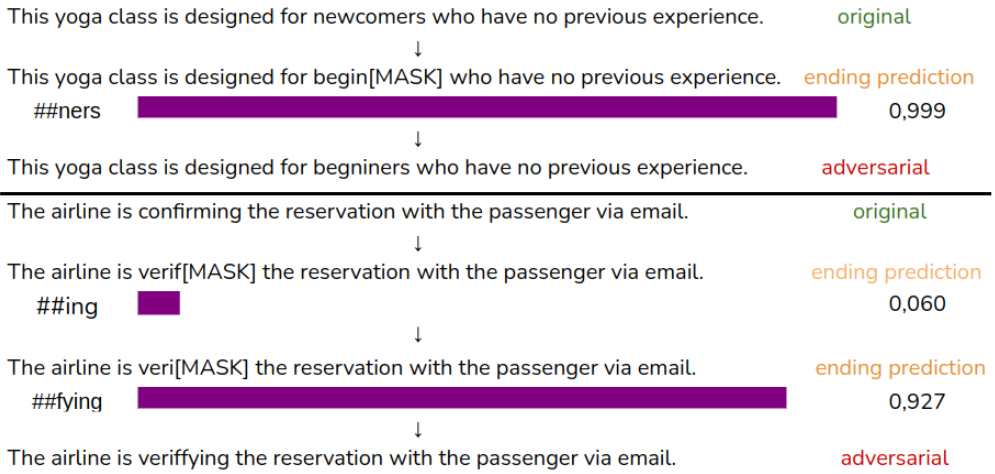
\includegraphics[width=\textwidth]{pictures/AdversialWord.png}
    \caption{Иллюстрация встраивания синонима в контекст}
    \label{fig:enter-label}
\end{figure}